% Chapter 3: Chapter 3. Methodology

\section{System Architecture Overview}\label{sec:3_1}

The system architecture integrates a RISC-V E203 Hummingbird v2 processor core with a custom CNN accelerator through the NICE coprocessor interface. Figure~\ref{fig:3_1} shows the top-level block diagram of the complete SoC.

\begin{figure}[htbp]
\centering

\includegraphics[width=0.85\textwidth]{figures/fig3_1_soc_architecture.png}
\caption{System-level block diagram of the E203 SoC with the CNN NICE accelerator.}
\label{fig:3_1}
\end{figure}

The E203 core is a 32-bit, 2-stage in-order RISC-V processor implementing the RV32IMAC instruction set. It provides a complete memory subsystem including an instruction tightly-coupled memory (ITCM) mapped at 0x8000\_0000 and a data tightly-coupled memory (DTCM) mapped at 0x9000\_0000. Standard peripherals—the Core Local Interrupt Controller (CLINT), Platform-Level Interrupt Controller (PLIC), UART0, and GPIO—are connected through the system bus fabric.

The CNN accelerator does not occupy a memory-mapped address range. Instead, it communicates with the processor exclusively through the NICE interface, which extends the processor’s execution pipeline with custom datapath logic. This architectural choice was made for three reasons:

Low latency: Custom instructions execute within the processor pipeline, eliminating the round-trip delay of bus transactions.

Programming convenience: The accelerator is controlled through standard RISC-V assembly instructions rather than load/store operations to memory-mapped registers.

Simplified integration: No bus arbitration, address decoding, or memory protection logic is required for the accelerator interface.

The system runs from the ITCM during normal operation. On reset, the E203 core fetches the first instruction from the boot ROM (MROM) at address 0x0000\_0000, which contains a jump vector that redirects execution to the start of the user program in ITCM. The DTCM stores input data (weights, activations) and output results, which are loaded into the accelerator via the NICE custom instructions.

Table~\ref{tab:3_1} presents the address map of the system.

\begin{table}[htbp]
\centering
\caption{SoC address space map.}
\label{tab:3_1}
\begin{tabular}{lccc}
\hline
Peripheral & Address Range & Width & Description \\ \hline\hline
MROM (Boot) & 0x0000\_0000 & 32-bit & Boot ROM with reset vector \\ \hline
ITCM & 0x8000\_0000 - & 64-bit & Instruction memory (128 KB) \\ \hline
 & 0x8001\_FFFF &  &  \\ \hline
DTCM & 0x9000\_0000 - & 32-bit & Data memory (64 KB) \\ \hline
 & 0x9000\_FFFF &  &  \\ \hline
CLINT & 0x0200\_0000 & 32-bit & Core local interrupt controller \\ \hline
PLIC & 0x0C00\_0000 & 32-bit & Platform-level interrupt ctrl \\ \hline
UART0 & 0x1001\_3000 & 32-bit & Serial communication \\ \hline
\end{tabular}
\end{table}

\section{NICE Custom Instruction Design}\label{sec:3_2}

\subsection{The NICE Protocol}

The NICE (Nuclei Instruction Co-extension) interface is a standardized coprocessor extension mechanism provided by the E203 processor. Unlike a memory-mapped peripheral, the NICE interface integrates the accelerator directly into the processor’s execution stage. The interface consists of four logical channels:

Request channel: Carries the instruction word and source register operands from the processor to the accelerator.

Response channel: Returns the result value from the accelerator to the processor’s register file.

Memory request channel (optional): Allows the accelerator to initiate its own memory transactions.

Memory response channel (optional): Returns data for memory read requests initiated by the accelerator.

In this design, the memory channels are not used. All data transfers between the processor and the accelerator occur through register operands (rs1 and rs2), which avoids the complexity of bus mastering and keeps the accelerator control logic simple.

The request channel signals are summarized in Table~\ref{tab:3_2}.

\begin{table}[htbp]
\centering
\caption{NICE request and response channel signals.}
\label{tab:3_2}
\begin{tabular}{lccc}
\hline
Signal & Direction & Width & Description \\ \hline\hline
nice\_req\_valid & Core to Acc & 1 & Request valid strobe \\ \hline
nice\_req\_ready & Core from Acc & 1 & Accelerator ready for request \\ \hline
nice\_req\_instr & Core to Acc & 32 & Full instruction word \\ \hline
nice\_req\_rs1 & Core to Acc & 32 & Source operand 1 (from integer reg.) \\ \hline
nice\_req\_rs2 & Core to Acc & 32 & Source operand 2 (from integer reg.) \\ \hline
nice\_rsp\_valid & Core from Acc & 1 & Response valid strobe \\ \hline
nice\_rsp\_ready & Core to Acc & 1 & Processor ready to accept response \\ \hline
nice\_rsp\_rdat & Core from Acc & 32 & Result data written to destination reg. \\ \hline
\end{tabular}
\end{table}

The handshake protocol uses a valid-ready mechanism on both channels. The request is a single-cycle pulse: the processor asserts nice\_req\_valid for exactly one clock cycle, and the accelerator captures the instruction and operands on the rising edge when nice\_req\_ready is also asserted. During computation, the accelerator de-asserts nice\_req\_ready to block new requests. When the result is ready, the accelerator asserts nice\_rsp\_valid and holds it until the processor responds with nice\_rsp\_ready.

\subsection{Instruction Encoding}

The six custom instructions use the RISC-V custom0 opcode (0x0B). Because the E203 NICE interface repurposes bits [14:12] as \{xd, xs1, xs2\} control flags rather than the standard funct3 field, the instruction differentiation is encoded entirely within the funct7 field (bits [31:25]).

Figure~\ref{fig:3_2} shows the instruction format.

\begin{figure}[htbp]
\centering

\includegraphics[width=0.70\textwidth]{figures/fig3_2_instruction_format.png}
\caption{RISC-V custom instruction format as interpreted by the E203 NICE interface.}
\label{fig:3_2}
\end{figure}

Table~\ref{tab:3_3} defines the six custom instructions.

\begin{table}[htbp]
\centering\small
\caption{NICE custom instruction set for the CNN accelerator.}
\label{tab:3_3}
\begin{tabular}{lp{1.8cm}p{1.8cm}p{2.8cm}p{3.5cm}}
\hline
Instruction & Encoding (hex) & Fields & Operands & Description \\ \hline\hline
CFG   & 0x0A00100B & funct7=5, xd=0, xs1=1, xs2=0 & rs1[0]=ReLU en & Configure accelerator \\ \hline
CLEAR & 0x0800000B & funct7=4, xd=0, xs1=0, xs2=0 & none & Clear PE accumulators \\ \hline
WLOAD & 0x0001800B & funct7=0, xd=0, xs1=1, xs2=1 & rs1=data, rs2=idx & Load weight column \\ \hline
DLOAD & 0x0201800B & funct7=1, xd=0, xs1=1, xs2=1 & rs1=data, rs2=idx & Load activation row \\ \hline
COMP  & 0x0400000B & funct7=2, xd=0, xs1=0, xs2=0 & none & Trigger MAC computation \\ \hline
RSTAT & 0x0600250B & funct7=3, xd=1, xs1=0, xs2=0 & rd=result & Read accumulator result \\ \hline
\end{tabular}
\end{table}

Figure~\ref{fig:3_2b} provides a visual summary of the complete NICE instruction set encoding.

\begin{figure}[htbp]
\centering
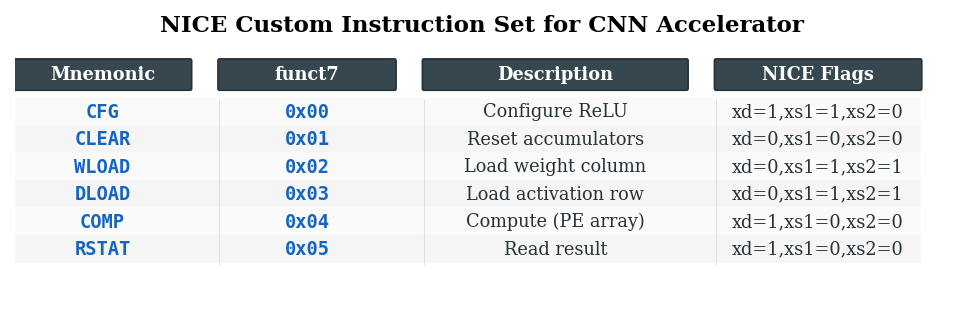
\includegraphics[width=0.85\textwidth]{figures/fig3_2b_instruction_table.png}
\caption{NICE custom instruction set for the CNN accelerator.}
\label{fig:3_2b}
\end{figure}

The key design decisions for this encoding are as follows.

WLOAD and DLOAD pack four INT8 values (32 bits total) into the rs1 register. The rs2 register supplies a 2-bit column/row index (0–3), selecting which group of four PEs to load. Over four consecutive WLOAD instructions, all 16 weight registers are filled; likewise, four DLOAD instructions fill all 16 activation registers.

COMP initiates parallel computation across the PE array. The accelerator checks that all four weight slots and all four activation slots have been loaded (via the w\_loaded\_mask and d\_loaded\_mask registers) before enabling the PE array. If either mask is incomplete, COMP returns an error.

RSTAT reads the final accumulated sum. The accelerator holds the result in a dedicated register and makes it available only after a COMP instruction has completed. Reading before COMP produces an error response.

CFG configures the optional ReLU (rectified linear unit) post-processing. When rs1[0] = 1, negative results are clamped to zero.

CLEAR resets all PE accumulators, the loaded mask registers, and the internal state machine to the idle state.

\subsection{Instruction Decode and Control Logic}

The NICE instruction decoder in cnn\_nice\_core.v inspects the funct7 field of the incoming instruction and generates the appropriate control signals. The Verilog code for the decoding logic is shown in Listing 3.1.

The decoder includes two error-checking mechanisms. First, if the instruction opcode is not 0x0B (custom0), the accelerator reports an error via nice\_rsp\_err. Second, for WLOAD and DLOAD instructions, the rs2 index is validated: only the lower two bits may be nonzero, ensuring the index is in the range [0,3].

The COMP instruction implements a guard condition: the accelerator asserts en\_pe only if all four weight-load and all four data-load operations have been completed, tracked by w\_loaded\_mask and d\_loaded\_mask. This prevents undefined behavior from partial data loading.

\subsection{Software Programming Model}

The accelerator is programmed through inline assembly macros. Listing 3.2 shows the C header file wrapper.

\begin{lstlisting}[language=C,style=cstyle]
// Listing 3.2: C-language wrapper macros for the NICE custom instructions.

#define CNN_CLEAR() do {                                         \
    __asm__ volatile(".insn r 0x0b, 0, 4, x0, x0, x0"           \
                     ::: "memory");                              \
} while(0)

#define CNN_WLOAD(data, idx) do {                                \
    __asm__ volatile(".insn r 0x0b, 0, 0, x0, %0, %1"           \
                     :: "r"(data), "r"(idx));                    \
} while(0)

#define CNN_DLOAD(data, idx) do {                                \
    __asm__ volatile(".insn r 0x0b, 0, 1, x0, %0, %1"           \
                     :: "r"(data), "r"(idx));                    \
} while(0)

#define CNN_COMP() do {                                          \
    __asm__ volatile(".insn r 0x0b, 0, 2, x0, x0, x0"           \
                     ::: "memory");                              \
} while(0)

#define CNN_RSTAT(result) do {                                   \
    __asm__ volatile(".insn r 0x0b, 0, 3, %0, x0, x0"           \
                     : "=r"(result));                            \
} while(0)
\end{lstlisting}

A typical convolution kernel follows a five-step sequence: (1) CLEAR to reset the accelerator state, (2) four WLOAD calls to load the weight columns, (3) four DLOAD calls to load the activation rows, (4) COMP to trigger computation, and (5) RSTAT to read the accumulated result. The data-flow pattern is described in detail in the next section.

\section{PE Array Architecture}\label{sec:3_3}

\subsection{Processing Element Microarchitecture}

Each processing element in the 4x4 array implements a single MAC operation on INT8 operands with INT32 accumulation. The PE is designed for output-stationary (OS) dataflow, meaning the partial sum is stored locally in the PE’s accumulator register.

Figure~\ref{fig:3_3} shows the PE datapath.

\begin{figure}[htbp]
\centering
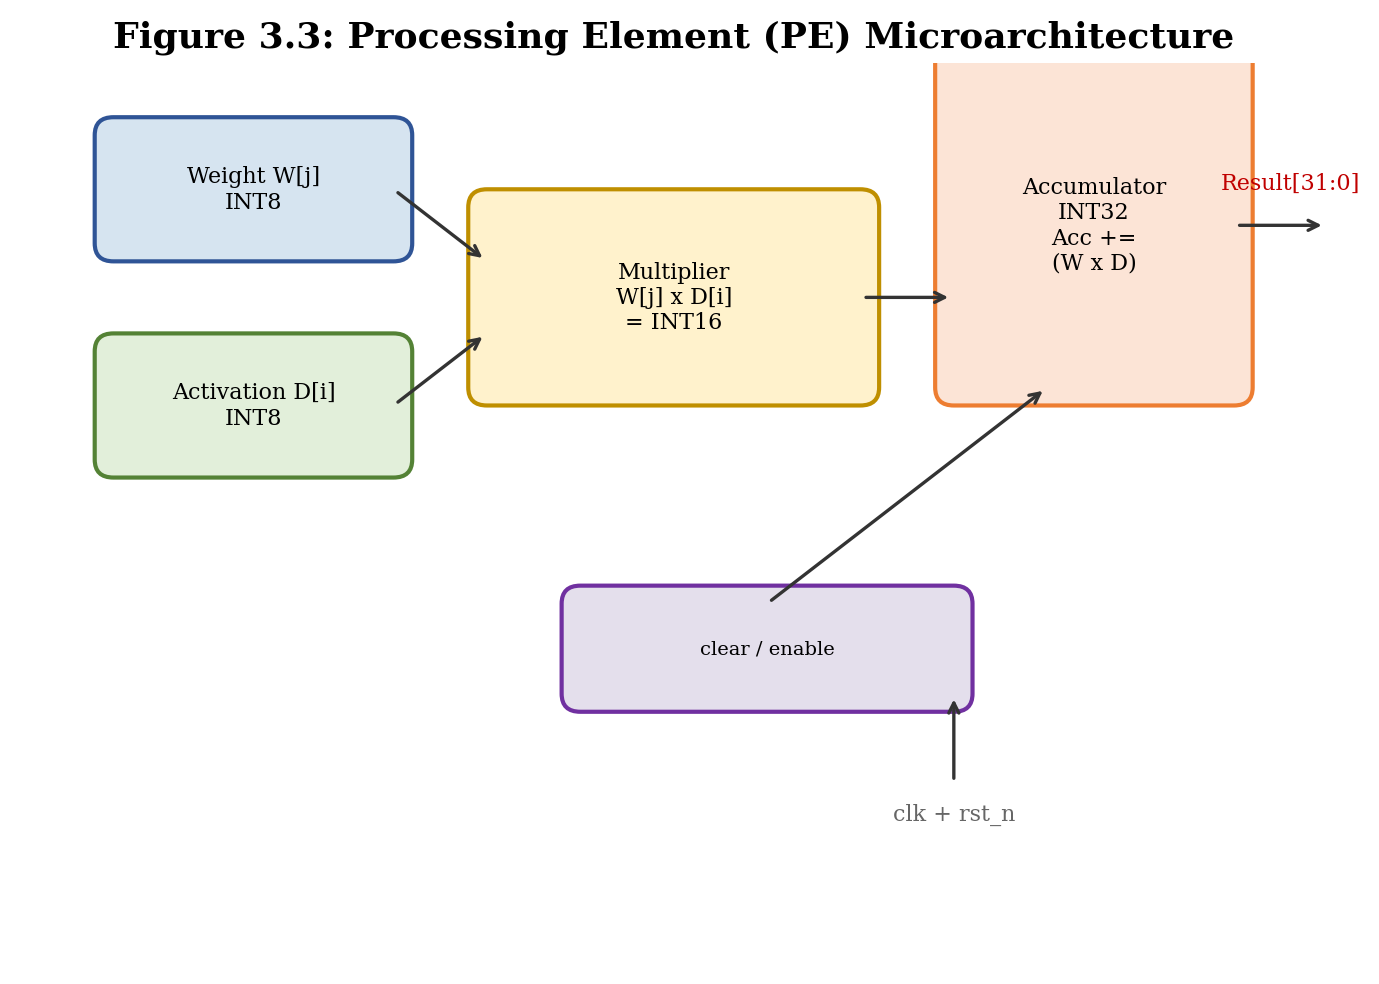
\includegraphics[width=0.60\textwidth]{figures/fig3_3_pe_microarchitecture.png}
\caption{Processing element microarchitecture showing the INT8 multiplier and INT32 accumulator.}
\label{fig:3_3}
\end{figure}

The PE RTL implementation is shown in Listing 3.3.

\begin{lstlisting}[language=Verilog,style=verilog]
// Listing 3.3: Single processing element (PE) implementation.
// Multiplies INT8 weight (w) by INT8 activation (d) and accumulates
// into a signed 32-bit register.

module pe(
    input                   clk,
    input                   rst_n,
    input                   acc_clr,
    input                   en,
    input  signed [7:0]     w,
    input  signed [7:0]     d,
    output reg signed [31:0] acc
);
    always @(posedge clk or negedge rst_n) begin
        if(!rst_n || acc_clr) begin
            acc <= 32'sd0;
        end else if(en) begin
            acc <= acc + (w * d);
        end
    end
endmodule
\end{lstlisting}

The accumulator supports two reset sources: a global rst\_n for power-on reset and an acc\_clr signal driven by the CLEAR instruction. The en signal, driven by the COMP instruction, gates the MAC operation. When en is de-asserted, the accumulator holds its current value, enabling multi-cycle accumulation across multiple COMP invocations if desired.

The signed multiplication w * d produces an INT16 intermediate result that is automatically sign-extended to INT32 by the addition operation, preventing overflow within a single MAC cycle. For multi-cycle accumulation across multiple convolution channels, the INT32 accumulator provides sufficient dynamic range: with 16 accumulated products, the maximum absolute sum is 16 x 127 x 127 = 258,064, well within the range of a 32-bit signed integer.

\subsection{Systolic Array Organization}

The 16 PEs are organized as a 4x4 grid. Each column shares a common weight value, and each row shares a common activation value. This organization maps directly to the computation of one output element in a 4x4 matrix multiplication: each PE computes the product of weight column i and activation row j, and the 16 products are summed to form the output.

Figure~\ref{fig:3_4} shows the array structure and the data distribution pattern.

\begin{figure}[htbp]
\centering

\includegraphics[width=0.70\textwidth]{figures/fig3_4_pe_array.png}
\caption{4x4 PE array organization showing weight column broadcast and activation row broadcast.}
\label{fig:3_4}
\end{figure}

The weight and activation storage within the PE array uses a column-wise and row-wise register file, implemented in pe\_array.v (Listing 3.4).

\newpage
\begin{lstlisting}[language=Verilog,style=verilog]
// Listing 3.4: PE array module showing weight and activation register file
// organization and the tree adder for the final sum.

module pe_array(
    input                   clk,
    input                   rst_n,
    input                   acc_clr,
    input                   en,
    input                   w_load,
    input                   d_load,
    input        [1:0]      vec_sel,
    input        [31:0]     w_in,
    input        [31:0]     d_in_packed,
    output signed [31:0]    out_sum
);
    reg signed [7:0] w_reg[15:0];
    reg signed [7:0] d_reg[15:0];
    wire signed [31:0] acc_out[15:0];

    generate
        for(i=0; i<16; i=i+1) begin : g_pe
            pe u_pe(clk, rst_n, acc_clr, en, w_reg[i], d_reg[i], acc_out[i]);
        end
    endgenerate

    always @(posedge clk or negedge rst_n) begin
        if(!rst_n) begin
            for(idx=0; idx<16; idx=idx+1) begin
                w_reg[idx] <= 8'sd0;
                d_reg[idx] <= 8'sd0;
            end
        end else begin
            if(w_load) begin
                case(vec_sel)
                    2'b00: {w_reg[3],  w_reg[2],  w_reg[1],  w_reg[0]}   <= w_in;
                    2'b01: {w_reg[7],  w_reg[6],  w_reg[5],  w_reg[4]}   <= w_in;
                    2'b10: {w_reg[11], w_reg[10], w_reg[9],  w_reg[8]}   <= w_in;
                    2'b11: {w_reg[15], w_reg[14], w_reg[13], w_reg[12]}  <= w_in;
                endcase
            end
            if(d_load) begin
                case(vec_sel)
                    2'b00: {d_reg[3],  d_reg[2],  d_reg[1],  d_reg[0]}   <= d_in_packed;
                    2'b01: {d_reg[7],  d_reg[6],  d_reg[5],  d_reg[4]}   <= d_in_packed;
                    2'b10: {d_reg[11], d_reg[10], d_reg[9],  d_reg[8]}   <= d_in_packed;
                    2'b11: {d_reg[15], d_reg[14], d_reg[13], d_reg[12]}  <= d_in_packed;
                endcase
            end
        end
    end

    assign out_sum = acc_out[0]  + acc_out[1]  + acc_out[2]  + acc_out[3]  +
                     acc_out[4]  + acc_out[5]  + acc_out[6]  + acc_out[7]  +
                     acc_out[8]  + acc_out[9]  + acc_out[10] + acc_out[11] +
                     acc_out[12] + acc_out[13] + acc_out[14] + acc_out[15];
endmodule
\end{lstlisting}

\subsection{Data Loading and Computation Schedule}

The NICE bus width is 32 bits, but the PE array requires 128 bits of weight data (16 x INT8) and 128 bits of activation data. To bridge this bandwidth gap, the loading is serialized across four cycles per data type.

The complete computation schedule is:

Table~\ref{tab:3_4} shows the computation schedule for one 4×4 matrix multiply-accumulate operation.

\begin{table}[htbp]
\centering
\caption{Computation schedule for one 4×4 matrix MAC operation.}
\label{tab:3_4}
\begin{tabular}{rll}
\hline
Cycle & Instruction & Description \\ \hline\hline
0 & CLEAR & Reset all PE accumulators and load mask registers \\ \hline
1 & WLOAD (col 0) & Load weight column 0 (4 INT8 values) \\ \hline
2 & WLOAD (col 1) & Load weight column 1 \\ \hline
3 & WLOAD (col 2) & Load weight column 2 \\ \hline
4 & WLOAD (col 3) & Load weight column 3 \\ \hline
5 & DLOAD (row 0) & Load activation row 0 (4 INT8 values) \\ \hline
6 & DLOAD (row 1) & Load activation row 1 \\ \hline
7 & DLOAD (row 2) & Load activation row 2 \\ \hline
8 & DLOAD (row 3) & Load activation row 3 \\ \hline
9 & COMP & Trigger parallel MAC across all 16 PEs \\ \hline
10 & RSTAT & Read accumulated INT32 result \\ \hline
\end{tabular}
\end{table}

The packed data format packs four INT8 values into one 32-bit word as shown in Figure~\ref{fig:3_5}.

\begin{figure}[htbp]
\centering

\includegraphics[width=0.65\textwidth]{figures/fig3_5_packed_format.png}
\caption{Packed INT8 data format within a 32-bit register for WLOAD and DLOAD.}
\label{fig:3_5}
\end{figure}

\subsection{Post-Processing: Optional ReLU}

After the computation completes and before the result is stored in the output register, an optional ReLU activation function is applied. The ReLU is implemented as a conditional multiplexer:

When relu\_en\_q is set (via the CFG instruction) and the result’s sign bit (bit 31) is 1, the output is clamped to zero. Otherwise, the raw accumulator sum is passed through unchanged.

\subsection{Resource Estimation}

The PE array resource footprint is dominated by the 16 MAC units. Table~\ref{tab:3_5} provides the estimated FPGA resource utilization.

\begin{table}[htbp]
\centering
\caption{Estimated FPGA resource utilization for the 4x4 PE array on an Artix-7 device.}
\label{tab:3_5}
\begin{tabular}{lccc}
\hline
Resource & Quantity & Width & Description \\ \hline\hline
Multiplier & 16 & 8 x 8 & Signed INT8 multiplication \\ \hline
Adder & 16 & 32-bit & Accumulation per PE \\ \hline
Weight regs & 16 & 8-bit & Distributed as flip-flops \\ \hline
Activation regs & 16 & 8-bit & Distributed as flip-flops \\ \hline
Accumulator & 16 & 32-bit & In each PE, registered \\ \hline
Tree adder & 1 & 32-bit & 16-input summation for final result \\ \hline
Control logic & \textasciitilde{}200 LUT & - & FSM, decoder, mask registers \\ \hline
\end{tabular}
\end{table}

\section{SoC Integration}\label{sec:3_4}

\subsection{Integration Hierarchy}

The CNN accelerator is integrated into the E203 SoC at the subsystem level. The e203\_subsys\_nice\_core module, which is the standard NICE integration wrapper provided by Nuclei, instantiates the cnn\_nice\_core module. This wrapper connects the NICE request/response signals between the E203 core and the accelerator.

The integration hierarchy is:

The NICE interface is activated by defining E203\_HAS\_NICE in the E203 configuration. When this macro is not defined, the e203\_subsys\_nice\_core module is not instantiated, and the accelerator is absent from the system.

\subsection{NICE Signal Connections}

The e203\_subsys\_nice\_core wrapper maps the E203 core’s NICE port signals to the accelerator’s ports. Listing 3.5 shows the wrapper instantiation.

\newpage
\begin{lstlisting}[language=Verilog,style=verilog]
// Listing 3.5: NICE subsystem wrapper instantiation (e203_subsys_nice_core.v).

module e203_subsys_nice_core (
    input                         nice_clk,
    input                         nice_rst_n,
    output                        nice_active,
    output                        nice_mem_holdup,
    input                         nice_req_valid,
    output                        nice_req_ready,
    input  [`E203_XLEN-1:0]       nice_req_inst,
    input  [`E203_XLEN-1:0]       nice_req_rs1,
    input  [`E203_XLEN-1:0]       nice_req_rs2,
    output                        nice_rsp_valid,
    input                         nice_rsp_ready,
    output [`E203_XLEN-1:0]       nice_rsp_rdat,
    output                        nice_rsp_err,
    // ... memory channel signals (unused) ...
);

    cnn_nice_core u_cnn_nice_core (
        .clk(nice_clk),
        .rst_n(nice_rst_n),
        .nice_req_valid(nice_req_valid),
        .nice_req_ready(nice_req_ready),
        .nice_req_instr(nice_req_inst),
        .nice_req_rs1(nice_req_rs1),
        .nice_req_rs2(nice_req_rs2),
        .nice_rsp_valid(nice_rsp_valid),
        .nice_rsp_ready(nice_rsp_ready),
        .nice_rsp_rdat(nice_rsp_rdat),
        .nice_rsp_err(nice_rsp_err),
        // Memory channel ports tied to 0/unused
    );
endmodule
\end{lstlisting}

The accelerator explicitly disables the NICE memory channels (nice\_mem\_holdup is tied to 0 and nice\_icb\_cmd\_valid is tied to 0), as all data transfer occurs through register operands.

\subsection{Memory Subsystem}

The processor boots from a 32-bit MROM containing a single jump instruction that redirects execution to the ITCM base address (0x8000\_0000). The ITCM is 64 bits wide and 16K entries deep (128 KB), connected to the processor through the instruction fetch unit. The DTCM is 32 bits wide and 16K entries deep (64 KB), connected through the load-store unit.

The ITCM and DTCM are initialized with Verilog hex files during FPGA bitstream generation. These hex files are produced by compiling a bare-metal C program, linking it to the appropriate memory regions, and converting the ELF binary to the text-format hex representation expected by \$readmemh. A critical implementation detail is that the hex file format must match the memory word width: ITCM (64-bit) requires 16 hex digits per line, while DTCM (32-bit) requires 8 hex digits per line.

\subsection{Peripheral Connections}

The SoC provides UART0 (connected to GPIO16 for RX and GPIO17 for TX at 115200 baud) as the primary debug output channel. The GPIO, CLINT, and PLIC peripherals are connected through the system bus fabric. The UART is initialized during the early boot sequence to enable printf-style debug messages. The GPIO module provides additional I/O capabilities, including the UART pin configuration.

\section{FPGA Bring-up Methodology}\label{sec:3_5}

\subsection{Build Flow}

The FPGA bitstream construction follows a two-stage build process. In the first stage, the bare-metal software program is compiled using the RISC-V GNU toolchain and converted to Verilog hex format for ITCM/DTCM initialization. In the second stage, Vivado synthesizes, places, and routes the RTL design with the memory contents pre-loaded from the hex files.

Figure~\ref{fig:3_6} shows the complete build pipeline.

\begin{figure}[htbp]
\centering

\includegraphics[width=0.85\textwidth]{figures/fig3_6_build_pipeline.png}
\caption{FPGA build pipeline from software compilation and RTL synthesis to bitstream generation.}
\label{fig:3_6}
\end{figure}

Several build modes are defined to support different validation scenarios:

bare\_metal: Minimal system without ILA probes, for final deployment.

bootvec\_sysclk\_ila: Includes ILA probes for CPU boot-chain debugging.

hello\_sysclk\_ila: Includes ILA probes and the hello\_e203 test program.

cnn\_sysclk\_ila: Includes ILA probes and the NICE accelerator test program.

Each build mode selects the appropriate top-level Verilog wrapper, ILA configuration, and memory initialization files through a PowerShell-based build script.

\subsection{ILA Probe Design}

The Integrated Logic Analyzer (ILA) is the primary on-chip debugging instrument. Seven probes, totaling 110 bits, are configured to capture key internal signals of the processor and accelerator:

\begin{table}[htbp]
\centering
\caption{ILA probe configuration.}
\label{tab:3_6}
\begin{tabular}{lccc}
\hline
Probe & Width & Signal Monitored & Debug Purpose \\ \hline\hline
probe0 & 32 & Program counter (PC) & CPU execution trace \\ \hline
probe1 & 4 & Reset and clock status & Verify clock tree and reset deassertion \\ \hline
probe2 & 3 & System memory bus activity & Detect bus transactions \\ \hline
probe3 & 32 & Memory command address & Identify which memory region is accessed \\ \hline
probe4 & 32 & Memory handshake counters & Quantify bus utilization \\ \hline
probe5 & 4 & UART TX state & Confirm UART transmission progress \\ \hline
probe6 & 3 & Debug/trap/stop flags & Detect processor exceptions \\ \hline
\end{tabular}
\end{table}

The ILA core is instantiated in a dedicated top-level wrapper module rather than being inserted post-synthesis via the Vivado GUI. This approach ensures that the probe signals are explicitly declared at the RTL level and survive synthesis without manual intervention. The trigger condition is configured to capture on the rising edge of the system clock, with a sample depth of 1024 cycles.

\subsection{Verification Strategy: Simulation-to-Hardware}

\begin{figure}[htbp]
\centering

\includegraphics[width=0.85\textwidth]{figures/fig_verification_chain.png}
\caption{Multi-stage verification flow from RTL simulation through FPGA board validation.}
\label{fig:3_7}
\end{figure}

The verification strategy employs a dual-track approach where RTL simulation and FPGA testing complement each other.

Simulation track (Icarus Verilog): The RTL design is verified with Icarus Verilog before any FPGA synthesis. The simulation testbench instantiates the SoC top module and drives the system clock and reset signals. A mock CPU testbench (tb\_cpu\_mock) provides standalone verification of the cnn\_nice\_core without requiring the full E203 processor, enabling faster iterations during accelerator development.

The simulation validates: 1. Normal path: CLEAR, four WLOADs, four DLOADs, COMP, RSTAT — the expected result is verified for known test vectors. 2. Error paths: COMP before loading all data, RSTAT before COMP. 3. Boundary conditions: Negative INT8 values (-128, -1), maximum positive values (127). 4. Reset behavior: Accumulators cleared after reset.

FPGA track (Vivado): After simulation passes, the design is synthesized for the Davinci Pro A7-100T FPGA (Artix-7 xc7a100t). The bring-up proceeds in stages:

Clock and reset verification: ILA captures clock activity and reset deassertion timing.

Boot chain validation: Processor PC is observed transitioning from MROM (0x0000\_0000) to ITCM (0x8000\_0000+), confirming correct boot vector execution.

UART output check: The hello\_e203 program sends three lines of output (“hello\_e203: boot”, “hello\_e203: uart ok”, “hello\_e203: loop”) at 115200 baud.

NICE instruction execution: The test\_nice assembly program exercises all six custom instructions. ILA captures verify that the CPU pipeline completes each NICE instruction and reaches the program completion point.

The simulation-to-hardware bridge proved critical for root-cause analysis. When the FPGA failed to boot, the exact same failing behavior was reproduced in simulation, which provided full signal visibility. The root causes—memory hex file formatting mismatch, missing Verilog macro definitions, and incorrect ILA probe placement—were all identified and fixed in simulation before rebuilding the FPGA bitstream.

\subsection{Debugging Methodology}

The debugging methodology follows a systematic isolation approach:

Observe: ILA captures the PC trace and key handshake signals.

Compare: The PC trace is compared against the disassembly listing of the compiled program to identify divergence points.

Isolate: Simulation reproduces the identical scenario with full waveform visibility, enabling probe of any internal signal.

Fix: The root cause is corrected in RTL, software, or build scripts.

Verify: Simulation passes the test case, and a new bitstream is built for FPGA confirmation.

This cycle typically requires 10–15 minutes per FPGA iteration (synthesis, place-and-route, bitstream generation) versus seconds for simulation. The simulation-first approach therefore maximizes engineering productivity by catching issues before the expensive FPGA build step.

